%(BEGIN_QUESTION)
% Copyright 2011, Tony R. Kuphaldt, released under the Creative Commons Attribution License (v 1.0)
% This means you may do almost anything with this work of mine, so long as you give me proper credit

Utløpstrykket fra dette vannfilteret reguleres av en PID-regulator som struper vannmengden som returneres til sumpen:

$$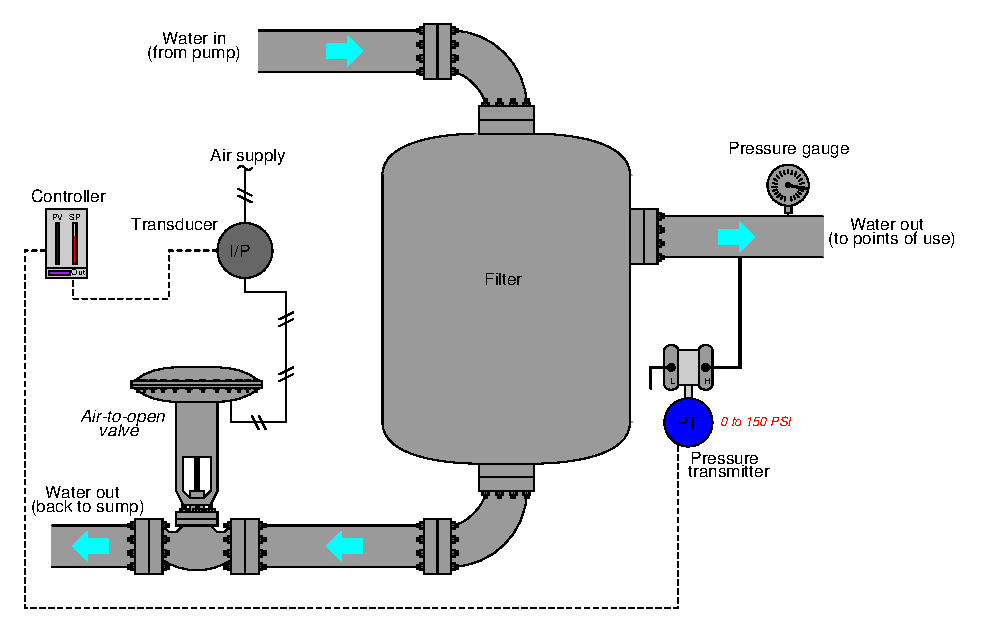
\includegraphics[width=15.5cm]{i00434x01.eps}$$

En operatør forteller at systemet har et problem: regulatorens frontpanel viser 146 PSI vanntrykk, med settpunkt på 100 PSI. Du legger merke til at stolpediagrammet for regulatorutgangen står på 100\%. En annen operatør i felt (nær varmeveksleren) melder over radio at reguleringsventilens spindel står i «lukket» posisjon, og at trykkmåleren på filterets utløpslinje viser 143 PSI.

\vskip 10pt

En annen instrumenttekniker er tilfeldigvis sammen med deg og anbefaler at dere kobler et multimeter på senderens signalledning for å måle 4-20 mA-signalet. Forklar hvorfor denne testen ville vært bortkastet tid, og foreslå en bedre test for å finne feilplasseringen.

\vskip 20pt \vbox{\hrule \hbox{\strut \vrule{} {\bf Forslag til sokratisk diskusjon} \vrule} \hrule}

\begin{itemize}
\item{} Et nyttig prinsipp i en slik feilsituasjon er {\it korrespondanse}: å identifisere hvilke feltvariabler som samsvarer med visningen på regulatorens frontpanel, og hvilke som ikke gjør det. Bruk denne sammenligningen på scenariet over, og forklar hvorfor den foreslåtte testen trolig ikke var det beste første steget.
\item{} Bestem riktig virkemåte for regulatoren i denne sløyfen (direkte eller revers).
\item{} For de som har studert PID-tuning: vurder kvalitativt passende P-, I- og D-parametere for sløyferegulatoren ut fra hvordan du forventer at denne prosessen responderer.
\end{itemize}

\underbar{file i00434}
%(END_QUESTION)





%(BEGIN_ANSWER)

Grunnen til at teknikerens foreslåtte test ville vært bortkastet tid er at regulatoren allerede viser et fornuftig trykk (omtrent det samme som feltmåleren). Med andre ord samsvarer regulatorens PV-indikasjon med trykkmåleren, noe som tyder på at det ikke er feil i inngangsdelen av reguleringssystemet.
 
%(END_ANSWER)





%(BEGIN_NOTES)

Regulatorens «beslutning» om å åpne returventilen helt gir mening siden PV $>$ SP. Det egentlige spørsmålet er derfor: «Hvorfor responderer ikke ventilen på regulatorutgangen?» Utgangsindikasjonen samsvarer ikke med ventilspindelens posisjon, noe som peker mot feil på FCE-siden (utgangssiden) av reguleringssystemet. Mulige feil er:

\begin{itemize}
\item{} Tap av instrumentluft til I/P-enheten
\item{} Avbrudd eller kortslutning i ledning mellom regulator og I/P
\item{} Stor luftlekkasje i ventilmembranen
\end{itemize}

Et godt «neste steg» er å inspisere ventilspindelens posisjon for å se om ventilen faktisk står helt åpen slik regulatoren kommanderer.

%INDEX% Basics, control loop troubleshooting: isolating area of fault by correspondence

%(END_NOTES)
